\section{Experimental results}
\label{sec:experimental_results}
In this section, we present experimental results using a low-power/low-cost sensor analytics application. As a use case, we present a CNN-regression model to predict x- y- coordinates of acoustic emissions based on piezoelectric vibrations. We compare quantitative and qualitative aspects of the analytics using floating-point 32-bit, fixed-point 8-bit, Hybrid-Logarithmic 6-bit, and Hybrid-Float6.

To demonstrate the proposed concept, we deploy the CNN model in the smallest Zynq SoC device for low-power inference. We compare the performance of the TP synthesized with standard FP (using Xilinx LogiCORE IPs) and Hybrid-Float6 design.

\subsection{Sensor Analytics Application}
The analytics model is designed to predict x- y- coordinates of acoustic emissions on a metal plate. The metal plate is in the presence of noise disturbance to simulate realistic conditions. In this subsection, we present the structure for experimental setup, data sets, and the CNN-regression model.

\subsubsection{Experimental Setup}
The experiment uses eight piezoelectric sensors (Vallen Systeme VS900) attached with magnetic holders on a metal plate (90 cm x 86.6 cm x 0.3 cm). The VS900 devices can operate either in active or passive mode. Six VS900 are used in passive mode as acoustic sensors and two in active mode to produce acoustic emissions. These acoustic emissions simulate anomalies on x- y- coordinates as well as the noise disturbance on the system. See \fig{fig:data_set}(a). To create data sets, the samples of acoustic emissions are labeled with their coordinates.

\subsubsection{Data Sets}
The data sets are recorded applying pulses on the metal plate, the x- y- coordinates of these pulses are used as labels. The pulses for training and validation data sets are shown in \fig{fig:data_set}(b) and \fig{fig:data_set}(c), respectively. The pulses for training and validation data sets are mutually exclusive, this exclusion is represented by the cross symbols in \fig{fig:data_set}(c). This creates a grid layout used to collect samples for the data sets. This grid is $10\times10$. This grid does not consider the four corners as they are used for magnetic holders.

\begin{figure}[t!]
	\centering
	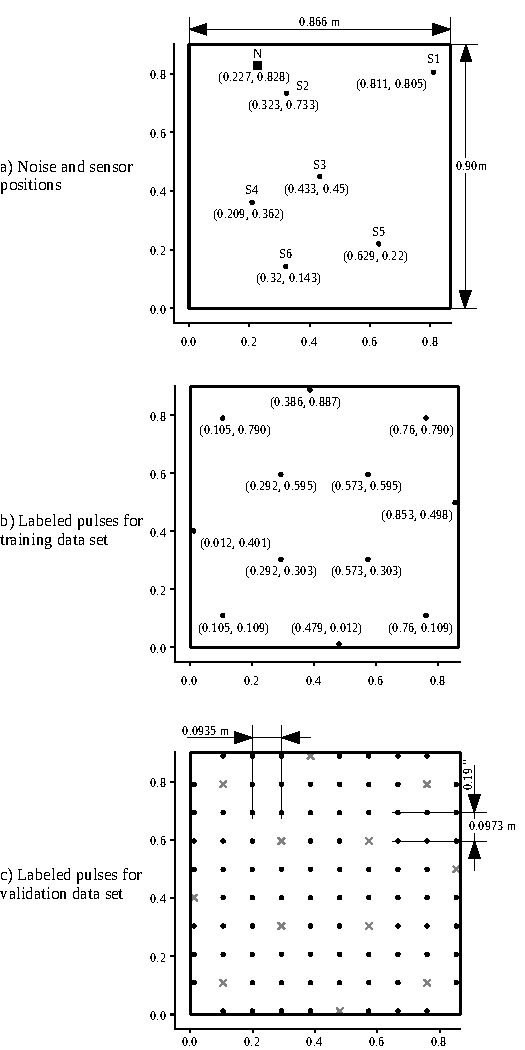
\includegraphics[width=\columnwidth]{../figures/histograms/data_set.pdf}
	\caption{Experimental setup for sensor analytics on structural health monitoring, all lengths are in meters (m).}
	\label{fig:data_set}
\end{figure}

In order to create reproducible acoustic emissions, we use 9-cycle sine pulse in a Hanning window with central frequency $f_\mathrm{c}$ (narrow-banded in the frequency domain). We assume guided Lamb waves based on the plate structure. The narrow-band behavior also reduces the dispersion of the acoustic emission waves~\cite{hannwindowsine}. The waveform can be expressed as a function of time $t$ as follows:

\begin{equation}
x_\mathrm{pulse}(t) = \frac{1}{2} \Big(1-\cos{\frac{f_\mathrm{c} t}{5}} \Big) A_0 \sin{f_\mathrm{c} t}.
\end{equation}

To generate the data sets, we use slightly different pulse amplitudes and frequencies for excitation. The pulse frequency $f_c$ is varied in 1 kHz steps between $\unit[300]{kHz}$ and $\unit[349]{kHz}$ and the amplitude $A_0$ is varied in $\unit[0.1]{V}$ steps between $\unit[2.6]{V}$ and $\unit[3.5]{V}$. This results in 500 different pulses for each of the excitation points.

The signals for labeled pulses and noise disturbance are generated by arbitrary waveform generators (AWGs). The sensor signals are recorded via a Vallen AMSY-6 measurement system with a resolution of 18 bits and a sampling rate of $f_\mathrm{S} =\unit[10]{MHz}$. The disturbance signal is gaussian noise with amplitudes between 0-3 V. This noise is applied via the piezoelectric device $N$ at $x=\unit[0.227]{m}$ and $y=\unit[0.828]{m}$, see \fig{fig:data_set}(a).

To obtain frequency components, the sampled pulses are converted into the frequency-time domain using the Short-Time Fourier Transform (STFT). This is calculated as follows~\cite{stft_lit}:

\begin{flalign}
\label{stft_eq2}
\mathcal{F}_{m,k}^\gamma= \sum_{n=0}^{N-1} x[n] \cdot \gamma^*[n-m\Delta M]\cdot \mathrm{e}^{\frac{-j 2 \pi k n }{N}}
\end{flalign}

Here $x[n]$ describes a discrete-time signal and $\gamma^*[n-m\Delta M]\cdot \mathrm{e}^{\frac{-j 2 \pi k n }{N}}$ the time- and frequency-shifted window function inside the considered interval $[0 , N-1]$. $\Delta M$ describes the time shift and $N$ the transformation window. Since only discrete frequencies and time points are considered, $m = 0,1,...,M-1$ is valid. For pictorial representation, the magnitude of the complex-valued STFT is employed in a spectrogram $\mathcal{S}_{m,k}$:

\begin{flalign}
\label{stft_eq3}
\mathcal{S}_{m,k}= \left|\mathcal{F}_{m,k}^\gamma\right|^2 = \left|\sum_{n=0}^{N-1} x[n] \cdot \gamma^*[n-m\Delta M]\cdot \mathrm{e}^{\frac{-j 2 \pi k n }{N}} \right|^2
\end{flalign}

In addition, these spectrograms are scaled in decibels. The spectrogram in decibels $\mathcal{S}_{m,k,\mathrm{dB}}$ results in $\mathcal{S}_{m,k,\mathrm{dB}}= 20 \cdot \mathrm{log}_{10}(\mathcal{S}_{m,k})$. For the conversion of the data, we use a signal length of 400 \textmu s (75 \textmu s pretrigger and 325 \textmu s post trigger). Thus, the arrival times of the pulses are included in the spectrogram for all channels and labeled positions. We use a Blackman window function~\cite{blackman_window}, a Fast Fourier Transform (FFT) length of 32 samples, and an overlap of 8 samples. The spectrograms are calculated for frequencies in the range of 100 kHz to 500 kHz. This results in a spectrogram size of 8x16 (8 frequency bins, 16 time values).

In order to generate larger data sets, we create four further variants with time shifts of 15 \textmu s/ 30 \textmu s/ 45 \textmu s/ 60 \textmu s. Subsequently, all spectrograms are converted to grayscale with scaling between -100dB and -40dB, see \fig{fig:spectrograms}.

In overall, the data set has a size of 1,440,000 images. This is the result of 500 (pulses) $\cdot$ 5 (spectrograms) $\cdot$ 6 (listening sensors) $\cdot$ 96 (excitation points).

\begin{figure}[t!]
	\centering
	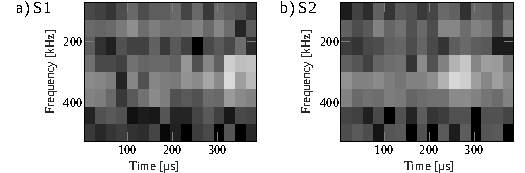
\includegraphics[width=\columnwidth]{../figures/histograms/spectrograms.pdf}
	\caption{Spectrograms of sensors $S_1, S_2$ converted to grayscale for pulses at $x =0.105$ m, $y = 0.109$ m with noise disturbance.}
	\label{fig:spectrograms}
\end{figure}

\subsubsection{CNN-Regression Model}
The data analytics is implemented with a CNN-regression model, see \fig{fig:model}. The structure of the model is described below:

\begin{enumerate}[label=\alph*)]
\item Input tensor. This is composed of spectrograms from the sensor signals. The tensor shape is defined by $S \times T \times F$, where $S$ is the number of sensors, and $T \times F$ is the time-frequency resolution of the spectrograms, see \fig{fig:model}(a).

\item Feature extraction. This is composed of three blocks of convolution, batch normalization, and max-pooling layers, see \fig{fig:model}(b). The number of channels in the convolution layers are defined by the hyper-parameters $A$, $B$, and $C$.

\item Regression function. This is an arbitrary function implemented with two fully connected layers and an output layer with linear activation, see \fig{fig:model}(c).
\end{enumerate}


\begin{figure}[t!]
	\centering
	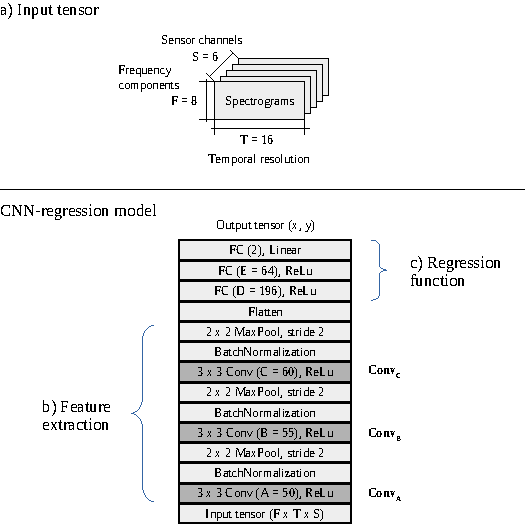
\includegraphics[width=\columnwidth]{../figures/models.pdf}
	\caption{CNN-regression model for sensor analytics.}
	\label{fig:model}
\end{figure}


\subsection{Training}
\subsubsection{Base Model}
The model in \fig{fig:model} is trained using Adam algorithm with iterative search. The Adam optimizer is configured with the default settings presented in \cite{kingma2014adam}: $\alpha = 0.001$, $\beta_1 = 0.9$, $\beta_2 = 0.999$, and $\epsilon = 1\mathrm{e}{-8}$. The training cycle patience is 10 iterations, the optimizer is executed with early stop patience of 10 epochs, and mini-batch size of 512 samples. This is applied using the method described in \Algo{alg:training} with $N_I = 10$, $N_E=10$, $B_{size}=512$.

The training results are illustrated in \fig{fig:optimization}(a). In this optimization, the initial and the final models achieve $MSE=\unit[0.0135]{m^2}$ and $MSE=\unit[0.0122]{m^2}$, respectively. The $MSE$ is calculated with the Euclidean distance (loss) between the expected and the predicted coordinates. The initial model is obtained at the first early stop (after 10 epochs). In each stop, the moving averages of the Adam optimizer get re-initialized. This facilitates searching for better local minima. The model gets saved/updated when finding a better minimum.

\begin{figure}[h!]
	\centering
	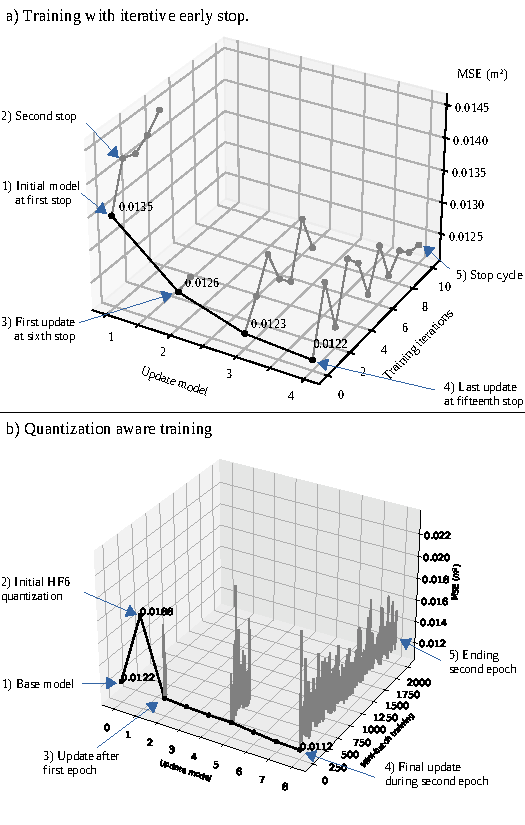
\includegraphics[width=\columnwidth]{../figures/histograms/training_and_quantization.pdf}
	\caption{Training results.}
	\label{fig:optimization}
\end{figure}

The final model achieves $MSE=\unit[0.0122]{m^2}$, which corresponds to $MAE=\unit[0.0955]{m}$. See \fig{fig:model_evaluation}(a). In total, the training takes 379 epochs in 25 cycle-search iterations. The first search takes 43 epochs for the initial model and subsequent search iterations take an average of 14 epochs. The total time is 53 minutes using a PC with AMD Ryzen 5 5600H and NVIDIA GeForce RTX 3050.

\begin{figure}[h!]
	\centering
	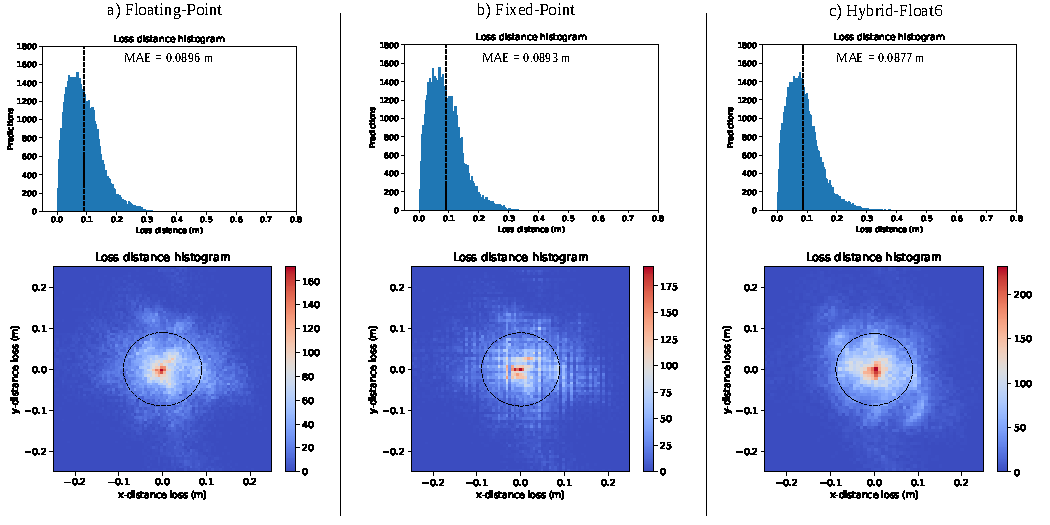
\includegraphics[width=\columnwidth]{../figures/histograms/model_evaluation.pdf}
	\caption{Performance of the model with different data representations.}
	\label{fig:model_evaluation}
\end{figure}

\subsubsection{TensorFlow Lite 8-bit quantization}
This integer quantization is an optimization method that converts 32-bit FP numbers (such as weights and activations) to 8-bit fixed-point numbers. This quantization scheme allows inference to be carried out using integer-only arithmetic\cite{hannwindowsine}.

The base model is quantized using the TensorFlow Lite library with integer-only quantization settings. The filter and bias tensors are represented by 8-bit and 32-bit signed integers, respectively. The input and output activation tensors are represented by 8-bit signed integer. For convolution layers, this quantization includes two additional tensor coefficients (output-multiplier and output-shift). These tensors are the same shape as the bias tensor and represented by 32-bit signed integers as well.

The fixed-point model achieves $MSE=\unit[0.0122]{m^2}$ and $MAE=\unit[0.0952]{m}$. See \fig{fig:model_evaluation}(b). The MAE obtains a reduction of 0.31\% compared to the base model. We attribute this to the regularization effect.

\subsubsection{Quantization Aware Training for Hybrid-Float6}
The QAT is a post-training step. We run this method during two epochs with mini-batch size of 10 samples with 4-bit exponent and 1-bit mantissa as parameters. This is applied using the method described in \Algo{alg:quantization_integration} with $N_{ep}=2$, $B_{size}=10$, $E_{size}=4$, $M_{size}=1$.

The QAT is illustrated in \fig{fig:optimization}(b). First, the model gets quantized with HF6 format before starting QAT, this obtains $MSE=\unit[0.0188]{m^2}$ and $MAE=\unit[0.1232]{m}$. This illustrates the inference of the base FP model (without QAT) on HF6 hardware. See \fig{fig:model_evaluation}(c). Then, after QAT, the final model achieves $MSE=\unit[0.0112]{m^2}$ and $MAE=\unit[0.0919]{m}$. This corresponds to an error reduction of 8.2\% and 3.77\%, respectively. See \fig{fig:model_evaluation}(d). The QAT time is 185 minutes.

\subsubsection{Quantization Aware Training for Hybrid-Logarithmic 6-bit}
For the sake of quality comparison, we generate the model with 6-bit logarithmic quantization on convolution parameters, see \fig{fig:floating}(e). This quantization matches the bit size of HF6. We run the QAT on the base model with hybrid logarithmic parameters. Then, the filter and bias tensors of convolution layers are represented by 6-bit signed logarithmic. This is applied using the method described in \Algo{alg:quantization_integration} with $N_{ep}=2$, $B_{size}=10$, $E_{size}=5$, $M_{size}=0$.

In this case, the model gets quality degradation. The model reaches $MSE=\unit[0.0123]{m^2}$ and $MAE=\unit[0.0968]{m}$, which correspond to an error increase of 0.82\% and 1.36\%, respectively. See \fig{fig:model_evaluation}(e).

A summary of inference with different data representations is presented in \fig{fig:model_evaluation}(f).

\subsection{Hardware Design Exploration}
The proposed hardware/software co-design is demonstrated on the Zynq-7007S system-on-chip (SoC) on the MiniZed development board. This SoC integrates a single ARM Cortex-A9 processing system (PS) and a programmable logic (PL) equivalent to Xilinx Artix-7 (FPGA) in a single chip \cite{xilinx2015zynq}. The Zynq-7007S SoC architecture maps the custom logic and software in the PL and PS, respectively.

In this platform, we implement the proposed hardware/software architecture to deploy the sensor analytics application. The desired model is converted to TensorFlow Lite (floating-point) and deployed on the SoC as a hex dump in a C array, this is used for the embedded software build. The Zynq-7007S SoC performs inference running TensorFlow Lite on the PS. The computational workload of convolution layers is delegated to the dedicated hardware.

\subsubsection{Benchmark on Embedded CPU}
We explore the performance of the embedded CPU for inference without hardware acceleration. In this case, TensorFlow Lite creates the CNN as a sequential model that allocates all computation to the CPU (ARM Cortex-A9) at $\unit[666]{MHz}$ and power dissipation of $\unit[1,187]{W}$.

The compute performance and run-time inference of the CPU are shown in \Tab{tab:performance}(a) and \fig{fig:runtime}(a), respectively.

\subsubsection{Benchmark on Tensor Processor with Standard Floating-Point Hardware using Xilinx LogiCORE IP}
For this design, we implement the TP with standard FP hardware prior synthesis. The design parameters are:
\begin{itemize}
	\item Max convolution kernel size: $K_W = K_H = 3$.
	\item Max input tensor width: $W_I = 16$.
	\item Max input and output channels: $C_I = 55$, $C_O = 60$.
	\item Filter and bias bit size: $BitSize_F=BitSize_B=32$.
	\item Input tensor bit size: $BitSize_I=32$.
\end{itemize}

Using equations from Section \ref{sec:memory_utilization}, the on-chip memory buffer utilization are $Input_M=84,480$b, $Filter_M=950,400$b, and $Bias_M=1,920$b. Hence, the required on-chip memory buffer size is $TP_B=1,036,800$b.

The post-implementation resource utilization and power dissipation are presented in \Tab{tab:resource_utilization}(a). The complete hardware platform utilizes 83\% of BRAM, this includes the on-chip memory requirements of the TP, DMA, and AXI interconnects. The total available on-chip memory (BRAM) on the Zynq-7007S SoC is 1.8Mb. The estimated power dissipation of the TP is $\unit[85]{mW}$ at $\unit[200]{MHz}$ (this estimation is provided by Xilinx Vivado).

\begin{table}[!h]\centering
	\caption{Resource utilization and power dissipation on the Zynq-7007S SoC.}\label{tab:resource_utilization}
	\scriptsize
	\begin{tabular}{lrrrrrr}\toprule
		\multirow{2}{*}{\textbf{TP engine}} &\multicolumn{4}{c}{\textbf{Post-implementation resource utilization}} &\multirow{2}{*}{\textbf{Power (W)}} \\\cmidrule{2-5}
		&\textbf{LUT} &\textbf{FF} &\textbf{DSP} &\textbf{BRAM 36Kb} & \\\midrule
		\multirow{2}{*}{(a) Floating-Point} &5,578 &8,942 &23 &41.5 &\multirow{2}{*}{1.429} \\
		&39\% &31\% &35\% &\textbf{83\%} & \\
		\multirow{2}{*}{(b) Hybrid-Float6} &7,313 &10,330 &20 &15 &\multirow{2}{*}{1.424} \\
		&51\% &36\% &30\% &\textbf{30\%} & \\
		\bottomrule
	\end{tabular}
\end{table}

The compute performance and inference schedule of the model on this hardware implementation are shown in \Tab{tab:performance}(b) and \fig{fig:runtime}(b), respectively. In this implementation, TensorFlow Lite delegates computation of \emph{Conv2D} tensor operations to the TP.

The implementation of the dot-product with standard FP engine (IEEE 754 arithmetic) utilizes proprietary multiplier and adder FP operator cores. Vivado HLS implements FP arithmetic operations by mapping them onto Xilinx LogiCORE IP cores, these FP operator cores are instantiated in the resultant RTL \cite{hrica2012floating}. In this case, the implementation of the dot-product with the standard FP computation reuses the multiplier and adder cores in different compute sections of the TP. The post-implementation resource utilization and power dissipation of the floating-point operator cores are shown in \Tab{tab:LogiCORE}.

\begin{table}[!t]\centering
	\caption{Compute performance of the CPU and TP on each Conv2D tensor operation. This table presents: tensor operation, computational cost in mega floating-point operations (MFLOP), latency, throughput, power efficiency, and estimated energy consumption as the energy delay product (EDP).}\label{tab:performance}
	\scriptsize
	\begin{tabular}{lrrrrrr}\toprule
		\textbf{Operation} &\textbf{MFLOP} &\textbf{t (ms)} &\textbf{MFLOP/s} &\textbf{MFLOP/s/W} &\textbf{EDP (mJ)} \\\midrule
		& &\multicolumn{4}{l}{\textbf{a) CPU (ARM Cortex-A9) @666MHz, 1.187 W}} \\
		Conv\textsubscript{A} &0.691 &112.24 &6.16 &5.19 &133.23 \\
		Conv\textsubscript{B} &1.584 &213.13 &7.43 &6.26 &252.99 \\
		Conv\textsubscript{C} &0.475 &46.59 &10.20 &8.59 &55.31 \\
		& &\multicolumn{4}{l}{\textbf{b) TP (Floating-Point engine) @200MHz, 85 mW}} \\
		Conv\textsubscript{A} &0.691 &12.49 &55.34 &651.11 &1.06 \\
		Conv\textsubscript{B} &1.584 &16.39 &96.66 &1,137.20 &1.39 \\
		Conv\textsubscript{C} &0.475 &3.59 &132.44 &1,558.13 &0.30 \\
		& &\multicolumn{4}{l}{\textbf{c) TP (Hybrid-Float6 engine) @200MHz, 84 mW}} \\
		Conv\textsubscript{A} &0.691 &6.92 &99.81 &1,188.24 &0.58 \\
		Conv\textsubscript{B} &1.584 &4.41 &358.94 &4,273.09 &0.37 \\
		Conv\textsubscript{C} &0.475 &0.99 &482.44 &5,743.29 &0.08 \\
		\bottomrule
	\end{tabular}
\end{table}

\begin{figure}[t!]
	\centering
	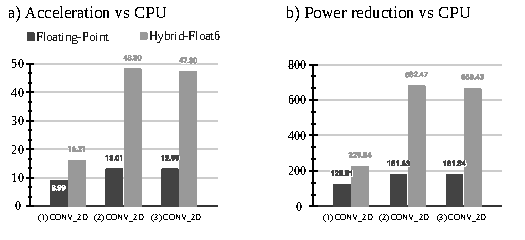
\includegraphics[width=1\columnwidth]{../figures/power_breakdown/acceleration_power_reduction.pdf}
	\caption{Inference acceleration and power reduction on the TP with floating-point and HF6 vs. CPU on the Zynq-7007S SoC.}
	\label{fig:acceleration}
\end{figure}


\begin{table}[!h]\centering
	\caption{Resource utilization and power dissipation of multiplier and adder floating-point (IEEE 754) operator cores (Xilinx LogiCORE IP).}\label{tab:LogiCORE}
	\scriptsize
	\begin{tabular}{lrrrrrr}\toprule
		\textbf{Core operation} &\textbf{DSP} &\textbf{FF} &\textbf{LUT} &\textbf{Latency (clk)} &\textbf{Power (mW)} \\\midrule
		Multiplier &3 &151 &325 &4 &7 \\
		Adder &2 &324 &424 &8 &6 \\
		\bottomrule
	\end{tabular}
\end{table}



\subsubsection{Tensor Processor with Hybrid-Float6 Hardware}
To demonstrate the proposed design, the TP with HF6 hardware restates the standard FP design parameters with the following customization for the FP 6-bit quantization in filter and bias: $BitSize_F=BitSize_B=6$.

Using equations from Section \ref{sec:memory_utilization}, the on-chip memory requirements are $Input_M=\unit[84,480]{b}$, $Filter_M=\unit[178,200]{b}$, $Bias_M=\unit[360]{b}$. Hence, the required on-chip memory buffer size is $TP_B=\unit[263,040]{b}$.

The post-implementation resource utilization and power dissipation are presented in \Tab{tab:resource_utilization}(b). The complete hardware platform utilizes 30\% of BRAM, this includes the on-chip memory requirements of the TP, DMA, and AXI interconnects. The estimated power dissipation of the TP is $\unit[84]{mW}$ at $\unit[200]{MHz}$ (this estimation is provided by Xilinx Vivado).

The compute performance and inference schedule of the model on this hardware implementation are shown in \Tab{tab:performance}(c) and \fig{fig:runtime}(c), respectively. \Fig{fig:acceleration} presents a comparison of the acceleration and the reduction of power dissipation between standard FP and HF6 hardware implementations.

This deployment does not require model parameter extraction/treatment. The 6-bit FP representation is wrapped into the standard FP. The dedicated hardware design extracts the 6-bit format automatically and performs computation.

\begin{figure}[t!]
	\centering
	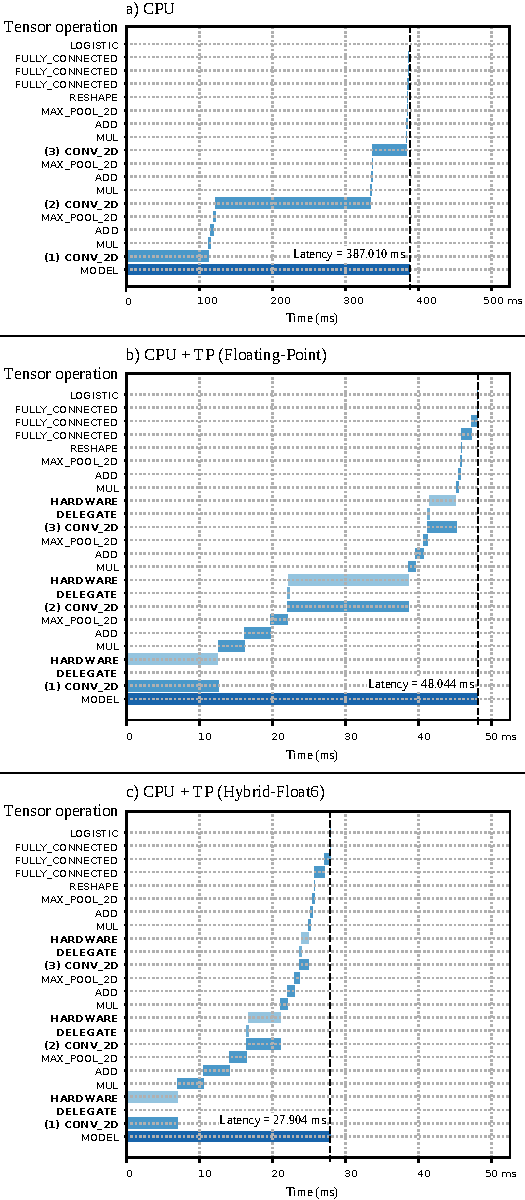
\includegraphics[width=1\columnwidth]{../figures/runtime/runtime.pdf}
	\caption{Run-time inference of TensorFlow Lite on the Zynq-7007S SoC. (a) CPU ARM Cortex-A9 at $\unit[666]{MHz}$, (b) cooperative CPU + TP with floating-point Xilinx LogiCORE IP at $\unit[200]{MHz}$, and (c) cooperative CPU + TP with Hybrid-Float6 at $\unit[200]{MHz}$.}
	\label{fig:runtime}
\end{figure}

\subsection{Discussion}
\subsubsection{Training and Quantization}
The training with iterative early stop obtains a model with enhanced accuracy than standard early stop. This method iteratively resets the moving averages of Adam's optimizer, which helps to find better local minima. This iterative search is suitable for models with low computational cost.

The TensorFlow Lite 8-bit quantization preserves the overall model accuracy. In some cases, the associated regularization effect can improve the accuracy. However, the error distribution in CNN linear regressions gets slightly degraded. \fig{fig:2d_error_distribtion}(b) shows this effect on three different models, where vertical and horizontal patterns appear in the error distribution of fixed-point quantization. We attribute this effect to the 8-bit resolution in the activation maps. In the case of HF6 quantization, the activation maps are represented by FP preventing this degradation.

The proposed 6-bit FP representation (E4M1) in convolution parameters improves latency, hardware area, and power dissipation, while preserving model accuracy. In our application, this number format produces better results than the 6-bit logarithmic representation (E5M0). This is demonstrated in \Fig{fig:model_evaluation}(d) and \Fig{fig:model_evaluation}(e).

Applying HF6 quantization on ALL-CNN-C \cite{springenberg2014striving} produces an accuracy degradation of 1.39\% and 0.11\% with QAT. While applying 6-bit logarithmic produces a degradation of 11.18\% and 7.22\% with QAT.

\begin{figure}[t!]
	\centering
	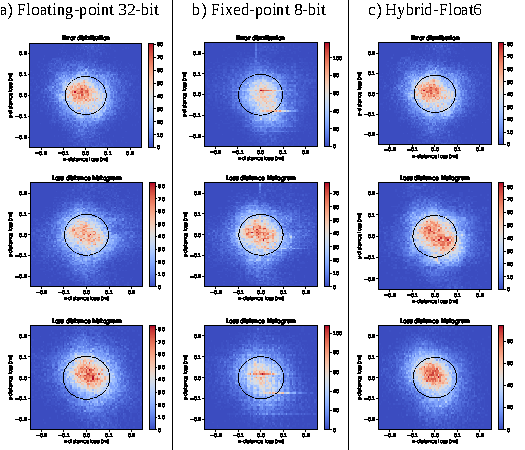
\includegraphics[width=1\columnwidth]{../figures/histograms/2D_error_distribtion.pdf}
	\caption{2D error distribution of three CNN-regression models.}
	\label{fig:2d_error_distribtion}
\end{figure}

\subsubsection{Implementation and Performance}
The proposed HF6 implementation reduces on-chip memory and DSP utilization while slightly increasing FF and LUT compared to the standard FP implementation. See \Tab{tab:resource_utilization} and \Fig{fig:resource_utilization}. The HF6 logic is implemented using FF and LUT, while the FP logic is implemented using Xilinx LogiCORE IPs with DSPs.

The compute performance of the CPU and TP on each convolution layer of the model is presented in \Tab{tab:performance} and \fig{fig:acceleration}. 
The peak acceleration and power efficiency of the TP with standard FP is $13\times$ and $1,558.13$ MFLOPS/s/W, respectively. The peak acceleration and power efficiency of the TP with HF6 is $48.3\times$ and $5,743.29$ MFLOPS/s/W, respectively. The HF6 hardware demonstrates an improvement of $3.7\times$ in acceleration and power efficiency with respect to the standard FP hardware. See \Fig{fig:acceleration}. The estimated power dissipation on the SoC is presented in \fig{fig:power}. This shows a very similar breakdown of power dissipation in both implementations. However, the energy efficiency is increased due to the reduced latency in HF6 hardware. A comparison of related work is presented in \Tab{tab:comparison}.

\begin{figure}[h!]
	\centering
	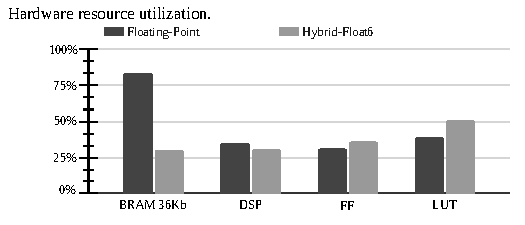
\includegraphics[width=1\columnwidth]{../figures/power_breakdown/resource_utilization.pdf}
	\caption{Hardware resource utilization on the Zynq-7007S SoC.}
	\label{fig:resource_utilization}
\end{figure}

\begin{figure}[h!]
	\centering
	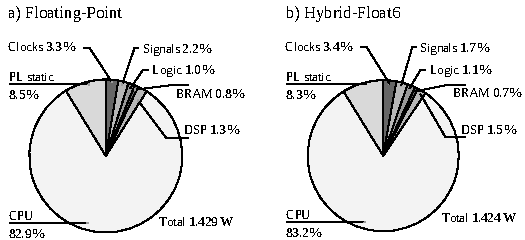
\includegraphics[width=1\columnwidth]{../figures/power_breakdown/power_breakdown.pdf}
	\caption{Estimated power dissipation on the Zynq-7007S SoC with PS at $\unit[666]{MHz}$ and PL at $\unit[200]{MHz}$.}
	\label{fig:power}
\end{figure}

The run-time inference of TensorFlow Lite on the SoC is illustrated in \Fig{fig:runtime}. This shows the convolution layers as the compute-bound operations. The proposed embedded platform is a cooperative system where the convolution operations are delegated to the dedicated hardware accelerator. The ARM CPU obtains a latency of $\unit[387]{ms}$ ($\unit[2.58]{FPS}$). The platform with standard FP hardware obtains a latency of $\unit[48]{ms}$ ($\unit[20.8]{FPS}$), while the implementation with HF6 obtains a latency of $\unit[27.9]{ms}$ ($\unit[35.84]{FPS}$). These represent an overall acceleration of $8\times$ and $13.87\times$ over the CPU, respectively.

For ML compatibility/portability, the 6-bit FP is wrapped into the standard FP representation. The dedicated hardware design extracts the 6-bit format automatically and performs the computation.

\subsubsection{SoC Design and Compatibility}
The proposed design is an alternative for low-power FP inference. The system runs as a cooperative hardware/software mechanism. This architecture delegates compute-bound tensor operations to a hardware accelerator.

The hybrid 32-bit FP and 6-bit FP quantization enables high quality of results and backward ML compatibility. Backwards ML compatibility gives portability from training to inference. This enables to run inference of HF6 quantized models on standard FP hardware and vise versa. Running inference of models without QAT allows rapid deployment; however, this will incur in accuracy degradation, see \Fig{fig:model_evaluation}(c).

\subsubsection{Future Work}
To reduce energy consumption, activation maps can be represented by Bfloat16. This would reduce hardware resource utilization, memory footprint, and data transfer. To increase performance, this implementation would require matching computational throughput with memory bandwidth using systolic arrays to replace the pipeline structure.
\begin{table*}[!t]\centering
	\caption{Comparison of hardware implementation with related work.}\label{tab:comparison}
	\scriptsize
	\begin{tabular}{lrrrrrr}\toprule
		Platform &Chunsheng Mei et al. \cite{mei2017200mhz} &Chen Wu et al. \cite{wu2021low} &BFP \cite{lian2019high} &Paolo Meloni et al. \cite{meloni2019cnn} &This work \\\midrule
		Device &XC7VX690T &XC7K325T &XC7VX690T &XC7Z007S &XC7Z007S \\
		Year &2017 &2019 &2019 &2019 &2022 \\
		Dev. kit cost &\$7,494 &\$1,299 &\$7,494 &\$89 &\$89 \\
		Format (activation/weight) &FP 16-bit &FP 8-bit / 8-bit &FP 16-bit / 8-bit &INT 16-bit &FP 32-bit / 6-bit \\
		Frequency (MHz) &200 &200 &200 &80 &200 \\
		Peak power efficiency (GFLOP/s/W) &18.72 &115.40 &82.88 &2.98 &5.74 \\
		Peak throughput (GFLOP/s) & 202.42 & 1086.8 & 760.83 &  10.62& 0.482\\
		Wall plug power (W) &10.81 &9.42 &9.18 &2.5 &2.3 \\
		BRAM 36Kb utilization &196.5 &234.5 &913 &44 &15 \\
		DSP utilization &1728 &768 &1027 &54 &20 \\
		\bottomrule
	\end{tabular}
\end{table*}